\documentclass[11pt]{article}
\usepackage{amsmath, amsfonts, amsthm, amssymb}  % Some math symbols
\usepackage{enumerate}
\usepackage{fullpage}
\usepackage{color}
\usepackage[x11names, rgb]{xcolor}
\usepackage{tikz}
\usepackage{graphicx}
\usepackage{listings}
\usepackage{fancyhdr}
\usepackage{pdflscape}
\usepackage[colorlinks = true,
             linkcolor = blue,
             urlcolor  = blue,
             citecolor = blue,
           anchorcolor = blue]{hyperref}

% usage: \fnurl{URL}{link text}
\newcommand\fnurl[2]{%
\href{#1}{#2}\footnote{\url{#1}}%
}

% \usepackage{fontspec}
% \setmainfont{Times New Roman}

\renewcommand*{\familydefault}{\sfdefault}

\setlength{\parindent}{0pt}
\setlength{\parskip}{6pt}
\pagestyle{empty}

\pagestyle{fancy}
\fancypagestyle{firststyle}
{%
  \lhead{\myname{} \\ \myandrew{} \\ \today \\ \vspace*{-.5em}}
  \rhead{15{-}221 \\ Fall 2014 \\ Section A \\ \vspace*{-.5em}}
  \setlength{\headsep}{50pt}
}

\fancypagestyle{zerostyle}
{%
  \renewcommand{\headrulewidth}{0pt}
}

\newcommand{\myname}{Justin Gallagher, Ted Li, Jacob Zimmerman, Howard Chen}
\newcommand{\myandrew}{Group 20}
\newcommand{\mytitle}{Progress Report}
\title{ExplainShell for Chrome \\ \vspace*{.5em} \Large\mytitle}
\date{}
%%%%%%%%%%%%%%%%%%%%%%%%%%%%%%%%%%%%%%%%%%%%%%%%%%%%%%%%%%%

\begin{document}
\pagenumbering{gobble}
\author{~\\
\normalsize {\bf Submitted to}\\
\normalsize Thomas M. Keating\\
\normalsize Assistant Teaching Professor\\
\normalsize School of Computer Science\\
\normalsize Carnegie Mellon University\vspace*{2em}\\
\normalsize {\bf Prepared by}\\
\normalsize Justin Gallagher\\
\normalsize Ted Li\\
\normalsize Jacob Zimmerman\\
\normalsize Howard Chen\vspace*{2em}\\
\normalsize School of Computer Science\\
\normalsize Carnegie Mellon University\\
\normalsize \today\\
\normalsize (Professor Keating granted us a two-day extension)
% ^ Is this necessary?
}

\clearpage\maketitle
\thispagestyle{firststyle}

\newpage
\lhead{\myname}
\rhead{\thepage}
\setlength{\headsep}{25pt}
\addtolength{\textheight}{-30pt}
\tableofcontents
\newpage
\pagenumbering{arabic}
\setlength{\voffset}{-50pt}
\setlength{\headsep}{25pt}

\section{Overview}

\subsection{Purpose}

This report intends to inform the client of our current progress in building
ExplainShell for Chrome. Specifically, we will cover additional information that
we have found relevant to our project, the goals we have accomplished, what we
still need to complete, required changes to our original procedure, and our plan
for finishing the project at the deadline. We will conclude with a discussion of
what exactly we expect to produce when finished.

\subsection{Project}

ExplainShell for Chrome is intended to help the user understand Unix shell
commands found online. With the aid of our Chrome extension, users will be able
to click on commands and be directed to the relevant \url{explainshell.com} page.
Our application eliminates the need to copy and paste the command into
\url{explainshell.com} and places a friendly reminder of ExplainShell's utility
in the reader's view. Combined, these two aspects eliminate the largest
barriers to people using \url{explainshell.com} freely, thus promoting its use.

As a complement to this utility, each click that users generate by following
links to \url{explainshell.com} from our Chrome extension will be sent off
anonymously to our ExplainShell Trends site, which will compile a database of
clicks which we will be able to query for statistics such as most recently
clicked commands, top referring sites and pages, most popular commands, and
more. Through this site, ExplainShell for Chrome users \textit{and others} will
be able to learn about new, helpful shell commands.

Thus, this system will both help bring attention to commands that users don't
understand as well as introduce them to new content generated by their peers.
It solves issues related to malicious code execution (because potential victims
will be more wary about running unknown commands), Unix shell education, and
community involvement.

\section{Literature Review}

We have found a number of reference materials useful along the development
process, mostly relating to the actual implementation of Chrome extensions and
web apps in Node.js. Of the sites we've visited, those that we document here
have been the most crucial to our current progress.

\subsection{Chrome Extension Developer Docs}

To get the ball rolling, we consulted the Chrome Extension Developer
documentation. There was a
\fnurl{https://developer.chrome.com/extensions/samples#search:contextmenus}%
{convenient starter extension} that in the end we only had to minimally tweak to
get the first version of our app working. Even though it was small, the
importance of this reference cannot be understated, because through it we
learned some best practices about writing Chrome extensions. These include
things like what pieces of metadata to include in the \texttt{manifest.json}
file and how best to structure our files and assets.

\subsection{Setting Up a Node.js Stack with Express \& MongoDB}

Setting up the backend ExplainShell Trends site turned out to be relatively
painless due to the comprehensiveness of
\fnurl{http://cwbuecheler.com/web/tutorials/2013/node-express-mongo/}{this
tutorial}. It went through the process of getting Node.js installed and getting
a simple app up and running. From here, we were able to adapt the site to our
needs, including setting up boilerplate pages for the landing and about
pages.

This tutorial also covered the process of setting up a local MongoDB instance,
which turned out to be incredibly straightforward. Using MongoDB, we were able
to begin populating the database with some sample data points for the purpose of
debugging.

\section{Progress}

We now present a general assessment of our progress so far. We will
also propose potential changes to our original schedule.

\subsection{General Assessment}
Up until this week, we have completed the development of Phase 1, 2, and 4.
So far, we have built a Chrome extension that parses and searches any web page
to identify any shell commands. As the extension finds any potential
commands using a set of heuristics, it will turn the original command text
into a clickable link, which will redirect the user to the corresponding
usage documentation at the ExplainShell website.

We have also completed the development of a back-end server that tracks
the commands that users search for using our extension. The server compiles
a database of clicks, which we will use to present various analytics,
including most recently visited commands, trending commands and top referring
sites.

The next step is to complete Phase 3, during which we will integrate the
front-end interface with the back-end server. To do this, we will likely need
to contribute to the existing ExplainShell code base to add in relevant APIs.

\subsection{Status}

Below is a general list of tasks that we have completed so far.
Note that the items listed below correspond to our original Gantt chart we
included in our initial proposal.
\begin{itemize}
  \item Create initial Chrome extension
  \item Test initial Chrome extension
  \item Parse page, add in external link
  \item Create in-page popup on hover (partially completed, see below
  for details)
  \item Setup basic analytics / trends site
  \item Add analytics support to back-end
\end{itemize}
Note that we have only partially completed the development of the in-page
popup. Our original proposal was to create a custom-styled popup to display
relevant information. This however would require us to first contribute to the
ExplainShell API, since we need to add in relevant API that allows us to
retrieve relevant reference documents from ExplainShell through web requests.
Therefore, the development of the in-page popup cannot be fully completed
before the ExplainShell API is available.

Therefore as of now, we have to temporarily compromise with an in-page popup
that uses an \texttt{iframe} web element to display the reference. This falls
short of our original proposal, since an \texttt{iframe} web element does not
allow us to customize the look and feel of the popup, and usually suffers from a
slower loading time.

As a reference of the work we have completed so far, please refer to
\fnurl{https://github.com/justingallagher/explainshell-for-chrome}{our GitHub
repository}. A rudimentary version of our Chrome extension is also available on
the
\fnurl{https://chrome.google.com/webstore/detail/explainshell-for-chrome/%
mhjgkgmolboemmbempmaapihlgcpomfi}{Chrome Web Store}.

\subsection{Projections}

Our project is slightly falling behind. This is partly due to the fact that
the time cycle of contributing to the ExplainShell open-source took longer
than we thought. We underestimated how long it would take to research the
technologies being used in the ExplainShell website (like Flask), and the length
of time required to gain a deep enough understanding of how the ExplainShell app
works. Since part of our project is dependent upon the integration of our code
into the ExplainShell code base, we may have to make a few adjustments to our
original schedule to deliver our final product on time.

To this end, we be making some adjustments to our original plan. Particularly,
if we cannot contribute to the ExplainShell code base by our project deadline,
we may need to compromise with our existing \texttt{iframe} solution for the
in-page popup, instead of using a custom-styled popup as proposed originally.

Our next major step would be to integrate the back-end logic with the
front-end. After the integration, our back-end server would be able to
track what users are searching for and provide relevant analytics. This also
would be the final portion of our project. We expect it to take one to two
weeks to complete.

\section{Recommendations}

Considering the above projections, we recommend the revised Gantt
chart seen in Figure~\ref{gantt}. It is given in context with a modified version of the old Gantt chart
that shows which tasks have been completed, dropped, and not finished.
\begin{center}
  \begin{figure}[h]
    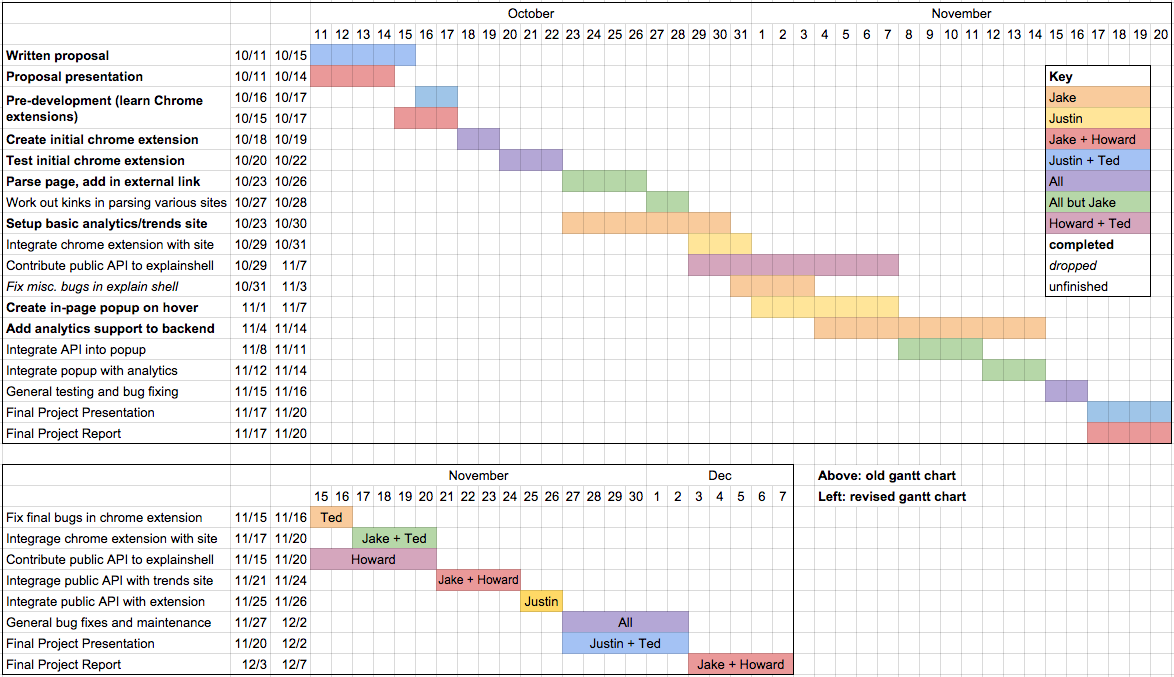
\includegraphics[width=\textwidth, keepaspectratio]{../gantt-chart-revised}
    \label{gantt}
    \caption{Revised Gantt chart, in context with progress on old Gantt chart}
  \end{figure}
\end{center}
As discussed earlier, these tasks are centered around resolving the two
bottlenecks to our current development: contributing to a public ExplainShell
API, and integrating it with the popup in our Chrome extension.

Once these tasks are done, we will be well on our way to finishing up the
project. The only thing that will need to be done after this is to collaborate
on the final project report and presentation, but by that time the only ongoing
development will be general maintenance.

\section{Discussion}

Unfortunately, we were unable to use our excess time to contribute back to the
ExplainShell repository fixing bugs and tidying up the code base. We had
allocated time to fix things like general bugs, but now we will only have enough
time to contribute a public API. This does not, however, interfere with the main
goals of the ExplainShell for Chrome project. It would have merely been a nice
gesture, considering that the ExplainShell app provides the core basis of
functionality to our project.

\end{document}
